\documentclass[
	hyperref={
		pageanchor=false,
		bookmarks=false,
		pdfpagelabels=false},
	% aspectratio=169,
	]{beamer}
\usepackage{pgfpages}									% for producing notes
\setbeameroption{show notes on second screen}
% \usetheme[progressbar=frametitle]{metropolis}           % Use metropolis theme
\useinnertheme{metropolis}
\useoutertheme[progressbar=frametitle]{metropolis}
\usecolortheme{metropolis}
\definecolor{lightblue}{RGB}{0,190,255}					% Define colors of corporate design of University of Stuttgart
\definecolor{midblue}{RGB}{0,81,158}
\definecolor{anthrazit}{RGB}{62,68,76}
\setbeamercolor{alerted text}{fg=midblue}				% Set colors
%\setbeamercolor{normal text}{fg=anthrazit}
\usepackage{caption}									% Use \captionof
\usepackage{tikz}
\usetikzlibrary{shapes,arrows}
\usepackage{amsmath}									% Use of align which is assumer superior to eqnarray
\usepackage{tabularx}									% Needed for using align in tabular-environment
\usepackage{array}										% Center text in column with specified width
\newcolumntype{P}[1]{>{\centering\arraybackslash}p{#1}}
% \usepackage{colortbl}									% Specify \arrayrulecolor for use in timeline
 \usepackage{booktabs}									% Use of \toprule
 \usepackage{tabu}
\usepackage{halloweenmath}

% \title{Application of Crowdsourcing}
% \subtitle{Learning \& Feedback}
\title{Application: Learning \& Feedback}
\date{October 31, 2017 $\pumpkin$}
\author{Andreas Poppele, Hyungyu Shin}
% \institute{KIXLAB, Korea Advanced Institue of Science and Technology}
%\logo{\includegraphics{images/unistuttgart_logo_de.jpg}}

\usepackage[T1]{fontenc} % utf8 <- produce real utf8 characters
\usepackage[utf8]{inputenc} % utf8 <- accept utf8 input characters
\usepackage[english]{babel}
\usepackage{anyfontsize} % mute warnings?
\usepackage{silence} % Error / Warning filter
\usepackage{textcomp} % Fix font warning
\usepackage[numbers]{natbib} % use natbib for \citeauthor{} and Co.

\makeatletter % Enable footnotes without marker
\def\blfootnote{\gdef\@thefnmark{}\@footnotetext}
\makeatother
%---------------------------------
% Silence Warning
%---------------------------------
\WarningFilter{biblatex}{Patching footnotes failed}
\WarningFilter{beamerthememetropolis}{You need to compile with XeLaTeX or LuaLaTeX to use the Fira fonts}

\NoHyper % remove warnings - but no links


\begin{document}
	\maketitle

	\begin{frame}
		\frametitle{Outline}
		\tableofcontents
	\end{frame}
\setlength{\belowcaptionskip}{-1.5em}

% Introduction; why is crowdsourcing predetermined for learning feedback?

%---------------------------------
% Section Learnersourcing Subgoal Labels for How-to Videos
%---------------------------------
\section{Subgoal labels for How-to videos}
	\begin{frame}{Motivation}
		Why learnersourced subgoal labels?
		\begin{itemize}
			\item<+-> Steps and subgoals support learning
			\item<+-> Millions of videos
			\item<+-> Prompts decrease misconceptions
		\end{itemize}
	\end{frame}

	\begin{frame}{Workflow}
		\begin{figure}
			\centering
			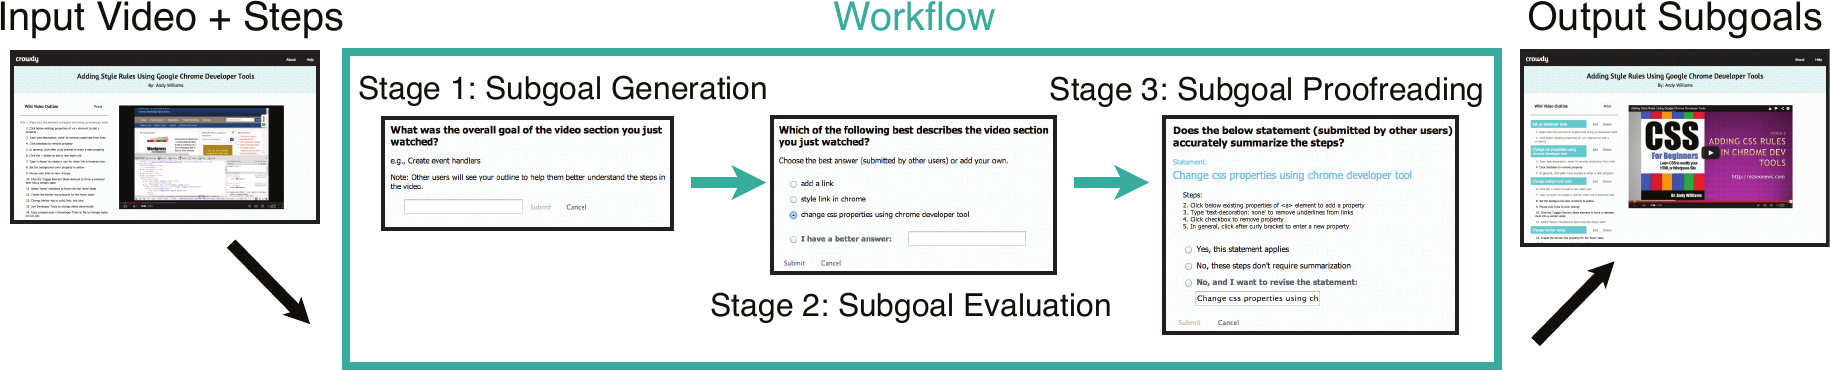
\includegraphics[width=\textwidth]{images/subgoal-workflow}
		\end{figure}
	\end{frame}

		\note{
			Stage 3: Necessary to adjust scope and language
		}

	\begin{frame}{Lessons learned}
		\begin{itemize}
			\item Don't interrupt too often
			\item Steps not necessary but considered helpful
			\item Ask question at every interval
		\end{itemize}
	\end{frame}

		\note{
			Lessons learned by pilot study
			\begin{itemize}
				\item Question interval; adaptive interval?
				\item less spam; users liked extra information
				\item avoid confusion
			\end{itemize}
		}

	\begin{frame}{Results}
		14 out of 17 labels voted matching or better than expert label.
	\end{frame}

	\begin{frame}{Challenges}
		\begin{figure}
			\centering
			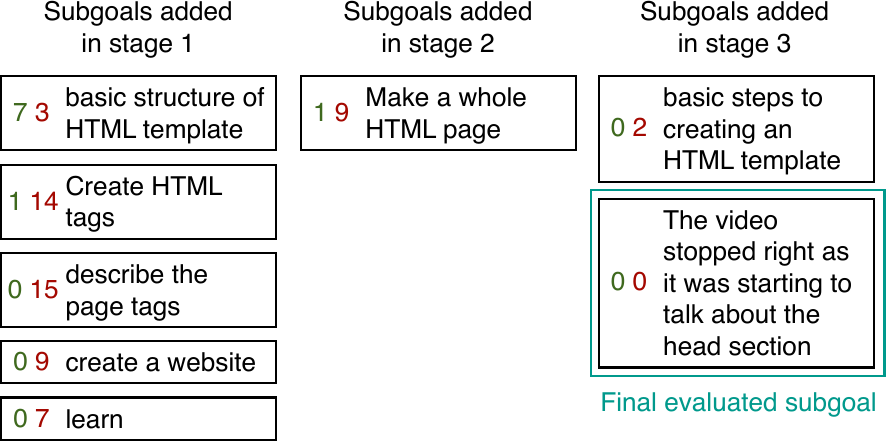
\includegraphics[width=0.7\textwidth]{images/subgoal-worsened}
		\end{figure}
	\end{frame}

		\note{
			Mediation method (only allow minor changes) + automatic evaluation
		}

%---------------------------------
% Section A User-Powered American Sign Language Dictionary
%---------------------------------
\section{American Sign Language Dictionary}

	\begin{frame}[standout]
		Please translate the words to english. You may use the internet.
	\end{frame}

		\note{
			Show some puppy images here?!
		}

	\begin{frame}{Motivation}
		\begin{itemize}
			\item<+-> American Sign Language (ASL) fourth most popular second language
			\item<+-> Looking up unknown signs is difficult 
		\end{itemize}
	\end{frame}

	\begin{frame}{How-to search}
		%TODO improve visual presentation
		\centering
		\begin{columns}
			\begin{column}{0.4\textwidth}<+->
				Search by example
				\begin{itemize}
					\item expensive
					\item inaccurate
				\end{itemize}
			\end{column}

			\begin{column}{0.5\textwidth}<+->
				Search by feature selection
				\begin{itemize}
					\item cumbersome
					\item poor implementation
				\end{itemize}
			\end{column}
		\end{columns}
	\end{frame}

		\note{
			Feature selection: omission of features not possible 
		}

	\begin{frame}{Proposed solution}
		\begin{figure}
			\centering
			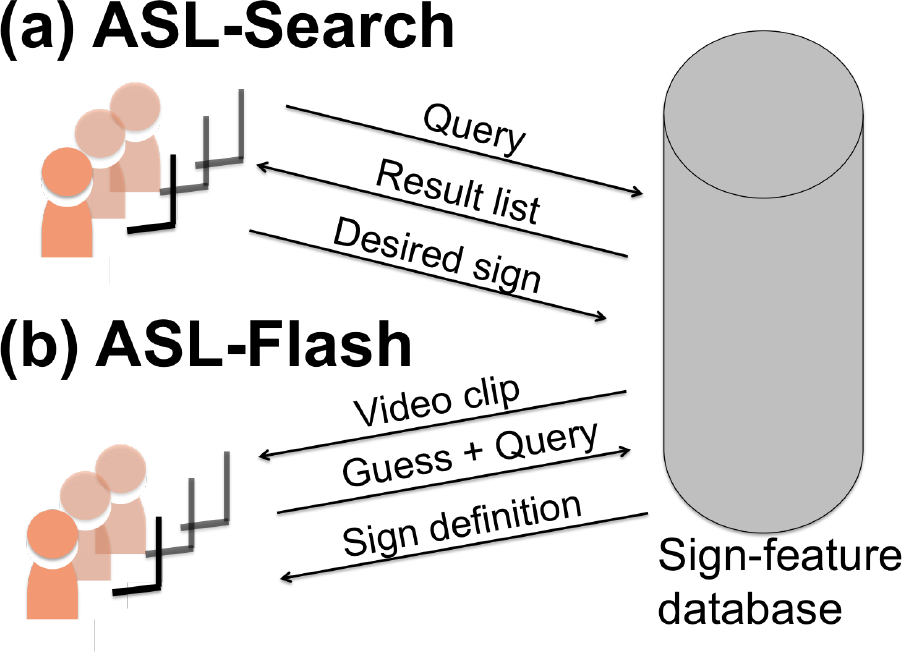
\includegraphics[width=0.7\textwidth]{images/ASL-overview}
		\end{figure}
	\end{frame}

		\note{
			Flash: Dual purpose

			Database: ML to improve matching
		}

	\begin{frame}{Search interface}
		\begin{figure}
			\centering
			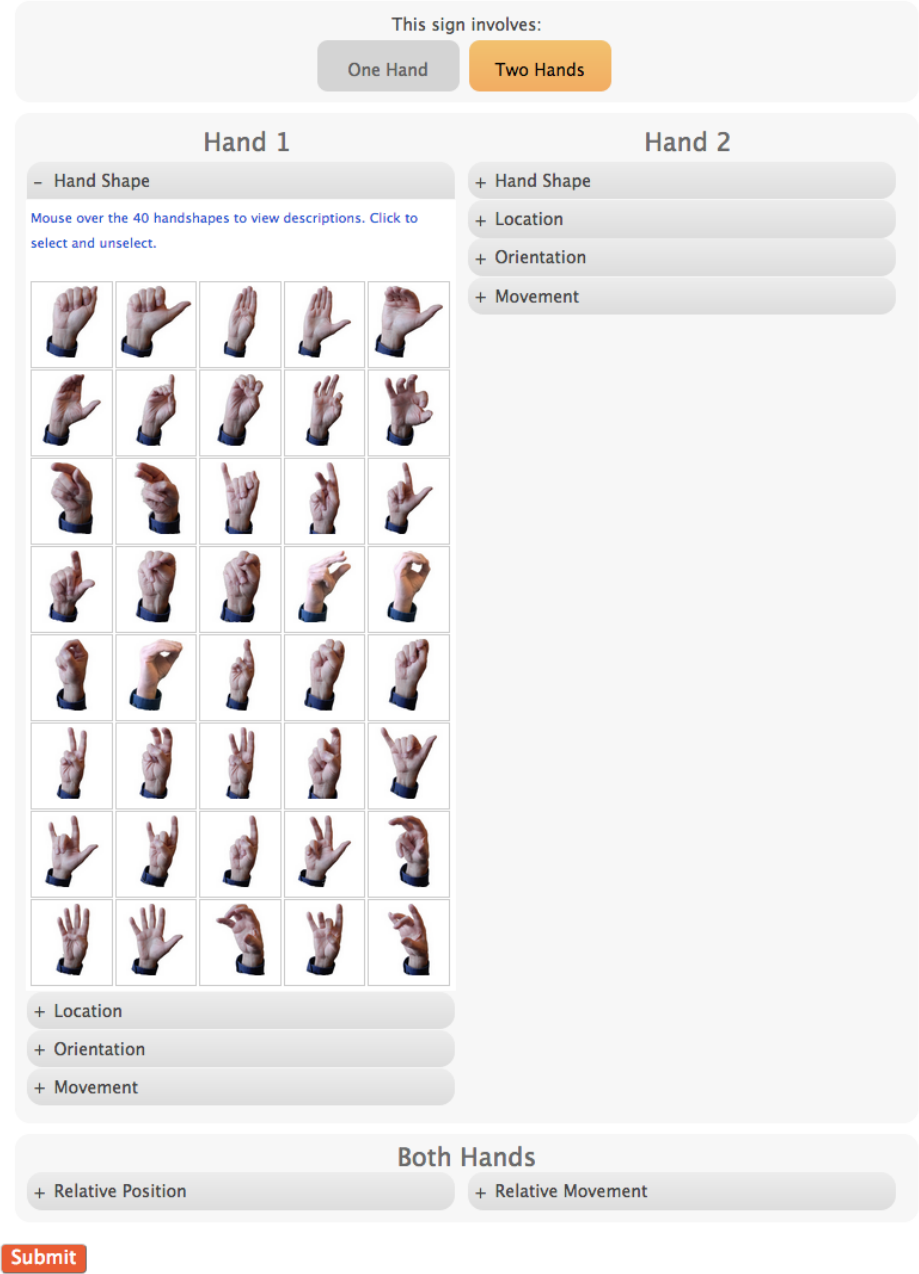
\includegraphics[height=0.9\textheight]{images/ASL-searchUI}
		\end{figure}
	\end{frame}

	\begin{frame}{Study results}
		\begin{figure}
			\centering
			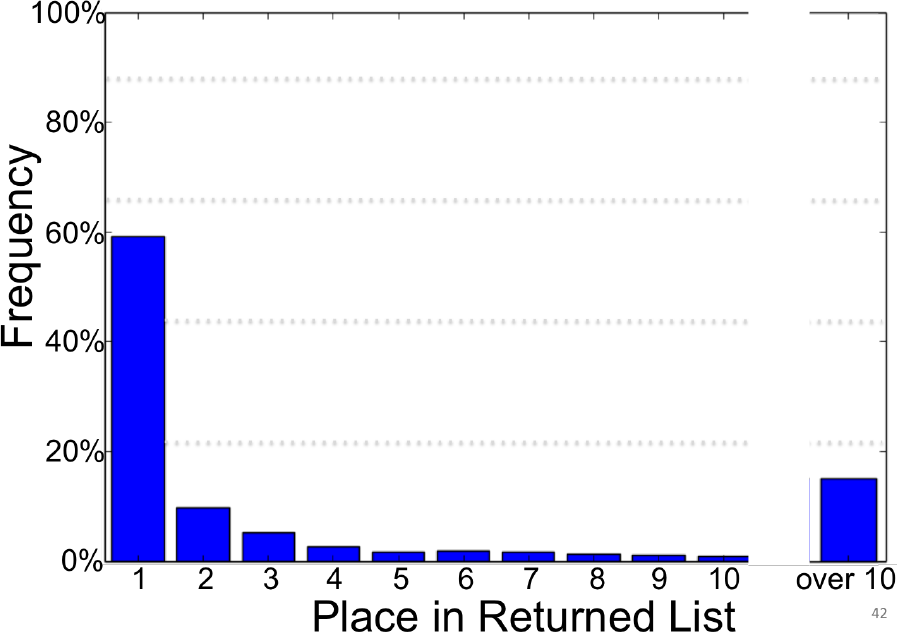
\includegraphics[width=0.8\textwidth]{images/ASL-results-placement}
			% 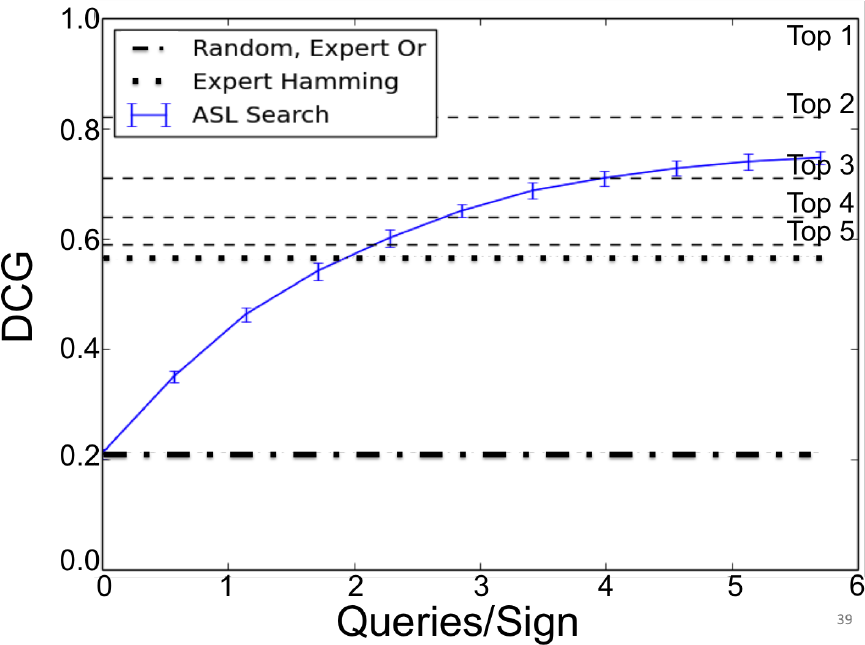
\includegraphics[width=0.8\textwidth]{images/ASL-results-progress}
		\end{figure}
	\end{frame}

		\note{
			670 queries by 94 users

			experienced valuable for learning

			80\% would use again

			85\% in top 10
		}


%---------------------------------
% Section Structuring, Aggregating, and Evaluating Crowdsourced Design Critique
%---------------------------------
\section{Crowdsourced Design Critique}	

	%IDEA present poorly designed poster (next paper boring; let's talk about my poster idea...)
	% please give me some feedback
	% you're feedback is bad
	% mine too...

	\begin{frame}{Motivation}
		\begin{itemize}
			\item Both-sided benefit when giving and receiving critique
			\item Useful feedback not always available
		\end{itemize}
	\end{frame}

		\note{
			\begin{itemize}
				\item domain-specific vocabulary
				\item rehearsing the mechanics of the crit process
			\end{itemize}
		}

	\begin{frame}{Giving critique}
		Helpful critique is $\dots$
		\begin{itemize}
			\item $\dots$conceptual.
			\item $\dots$specific.
			\item $\dots$actionable.
		\end{itemize}
	\end{frame}

		\note{
			\begin{itemize}
				\item help a student grasp the concept of a standard
				\item compare the actual level of performance with this standard
				\item engage in action that closes this gap
			\end{itemize}
		}

	\begin{frame}{CrowdCrit}
		\begin{figure}
			\centering
			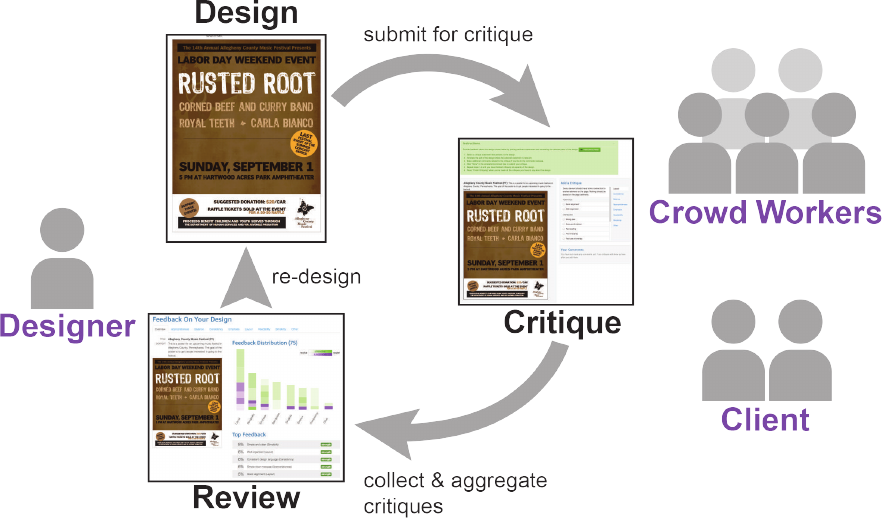
\includegraphics[width=0.9\textwidth]{images/CrowdCrit-overview}
		\end{figure}	
	\end{frame}

	\begin{frame}{Interface}
		\begin{figure}
			\centering
			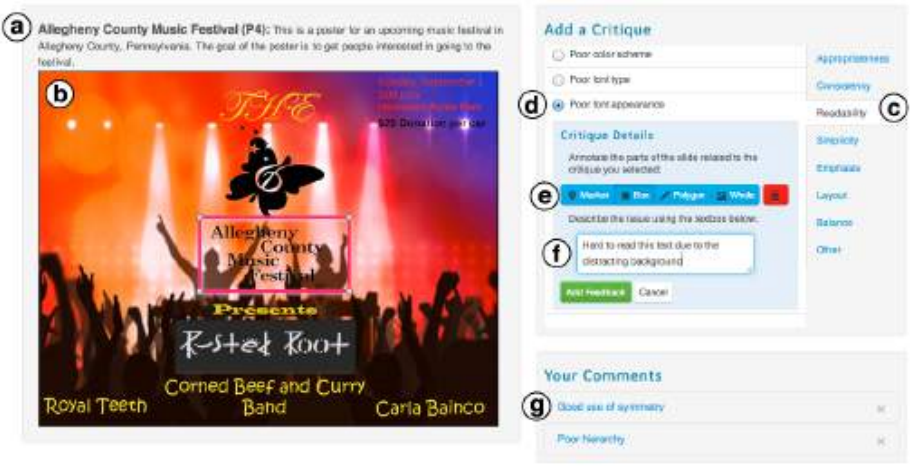
\includegraphics[width=0.9\textwidth]{images/CrowdCrit-critUI}
		\end{figure}
	\end{frame}

		\note{
			\begin{itemize}
				\item key design principles and critique statements
				\item critique statements includes description and generic solution
				\item highlight problem in design and give annotation
			\end{itemize}
		}

	\begin{frame}{Aggregation}
		\begin{figure}
			\centering
			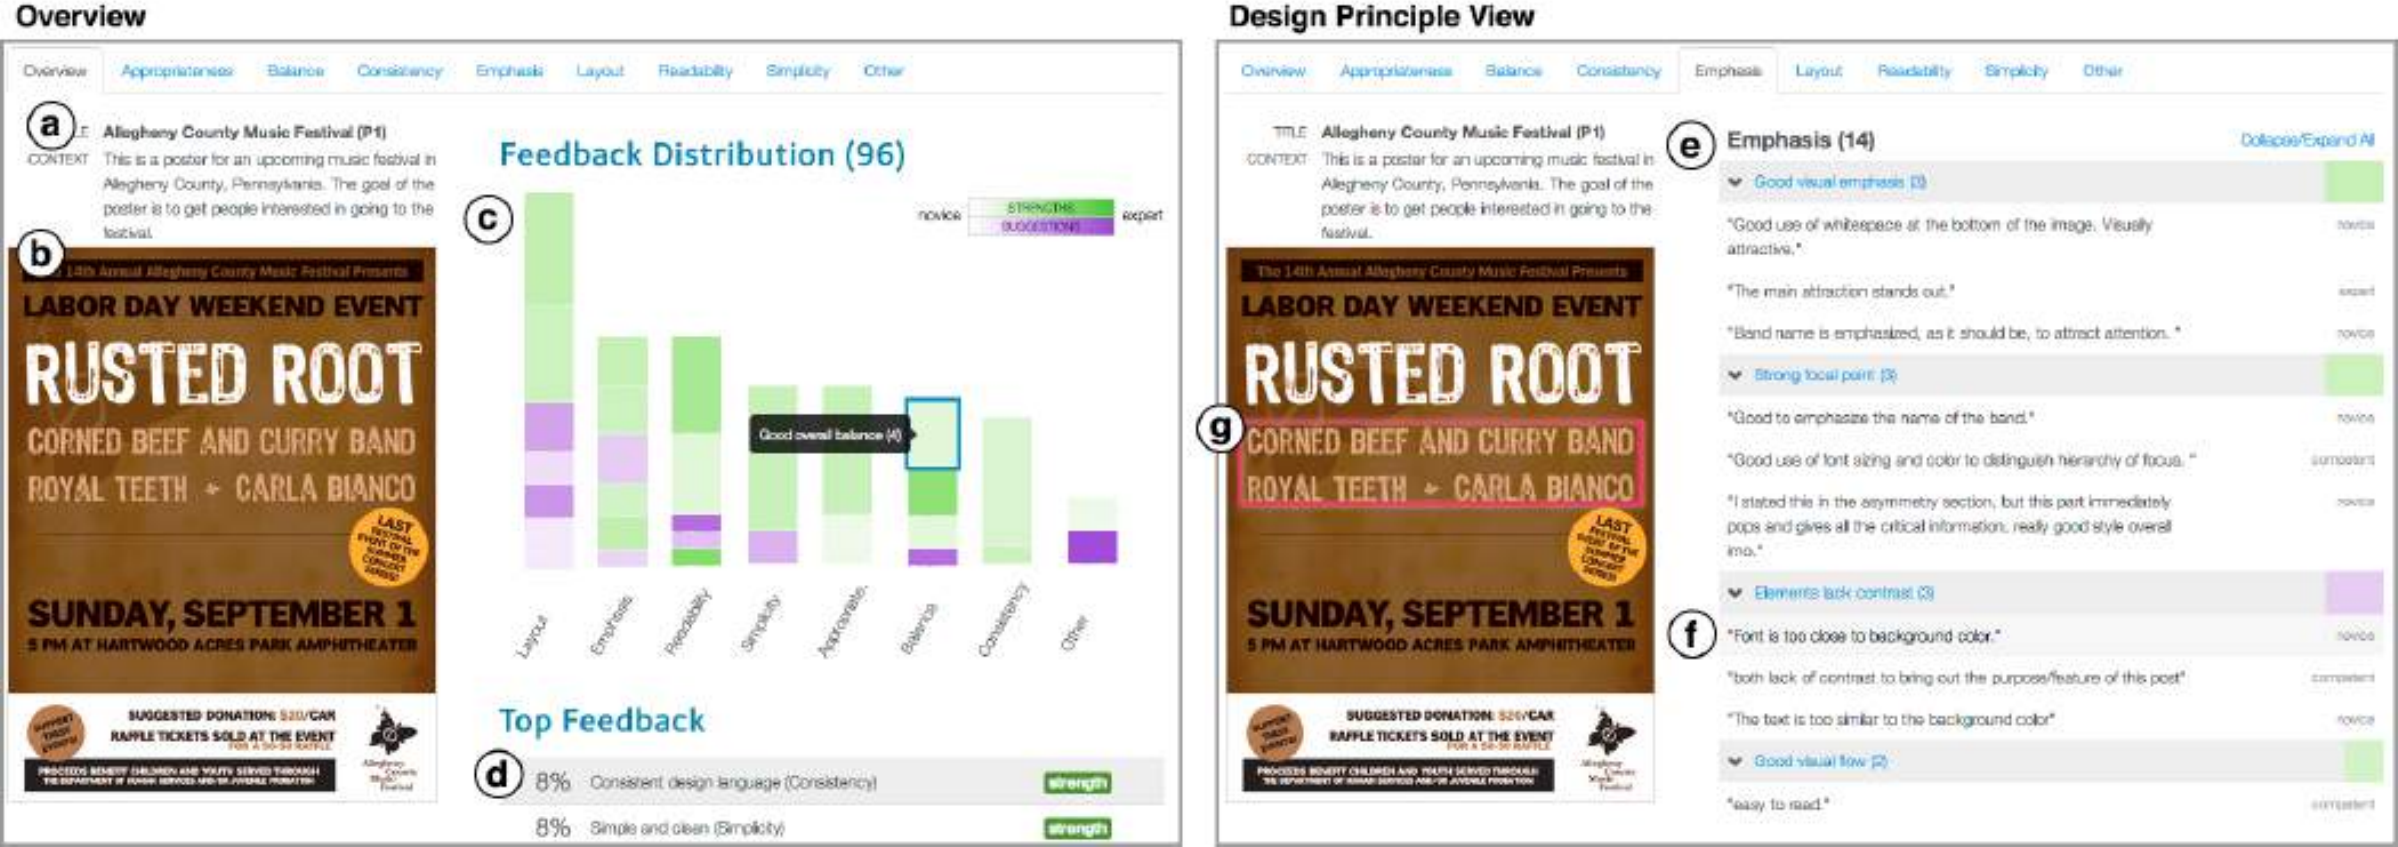
\includegraphics[width=\textwidth]{images/CrowdCrit-aggregation}
		\end{figure}
	\end{frame}

		\note{
			\begin{itemize}
				\item two views: overview + design principle
				\item presented in variable complexity
				\item positive -> green; negative -> red
				\item lighter -> less expertise
				\item Top Feedback
			\end{itemize}
		}

	\begin{frame}{Study results}
		\begin{itemize}
			\item<+-> Crowd workers and experts agreement of 45\% to 60\%
			\item<.-> Crowdsourced feedback is more rich
			\item<+-> Designers liked the interface
			\item<.-> Designers felt like the feedback is helpful
			\item<+-> No significant difference between crowd feedback and generic feedback
		\end{itemize}
	\end{frame}

		\note{
			\begin{itemize}
				\item three studies in total
				\item numerous, fast, too expensive though, nice interface
				\item maybe leads to concentrating on minor things
				\item platform doesn't engage big changes
			\end{itemize}
		}

%---------------------------------
% Questions
%---------------------------------
	\begin{frame}[standout]
		\begin{figure}
			\centering
			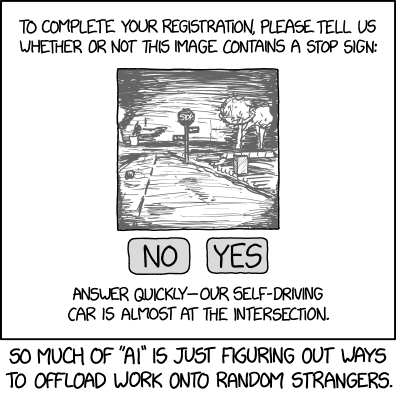
\includegraphics[width=0.7\textwidth]{images/self_driving}
			\label{fig:bad_note}
		\end{figure}
		xkcd.com
	\end{frame}

% \fontsize{6pt}{7.2}\selectfont
% \bibliographystyle{./aux/IEEEtranN}
% \bibliography{./aux/IEEEabrv,../ArbeitBib}

\end{document}
